\documentclass[landscape]{slides}
\usepackage[landscape, margin=2cm]{geometry}
\usepackage{color}
\usepackage{bm}
\usepackage{graphicx}
\usepackage{hyperref}
\graphicspath{ {./img/} {./charts/} }


\title{Show and Tell: Bits and Bobs}
\author{Adam Johnson - me@adamj.eu}
\date{31st July 2014}

\begin{document}

\maketitle


\begin{slide}

    \textcolor{blue}{\Large{Recap}}

    \begin{itemize}
        \item Given two talks:
        \item Calendar Lifelogging
        \item Skill Acquisition
        \item This talk is just a few little things as an update on things to show and tell
    \end{itemize}

\end{slide}


\begin{slide}

    \textcolor{blue}{\Large{What have I been up to?}}

    \begin{enumerate}
        \item Cycled Land's End to John O' Groats
        \item Improved Lifelogger process
        \item Using `Lift'
    \end{enumerate}

\end{slide}


% part 2


\begin{slide}

    \textcolor{blue}{\Large{Cycling from Land's End to John O' Groats}}

    \begin{itemize}
        \item 990 mile route, 14 days, with Dad, Brother, and Tour Group
        \item 8th to 21st June
        \item Aim for simple tracking, nothing fancy
    \end{itemize}

\end{slide}



\begin{slide}

    \textcolor{blue}{\Large{LEJOG Tracking Tools}}

    \begin{itemize}
        \item \textbf{Google Location History} - basic position/time data
        % as recommended by Jamie last time I was here
        \item \textbf{Garmin} - more precise distance/elevation statistics
        \item \textbf{Lifelog} - continued via some simple shortcuts
    \end{itemize}

\end{slide}


\begin{slide}

    \textcolor{blue}{\Large{LEJOG Map}}

    \begin{center}
        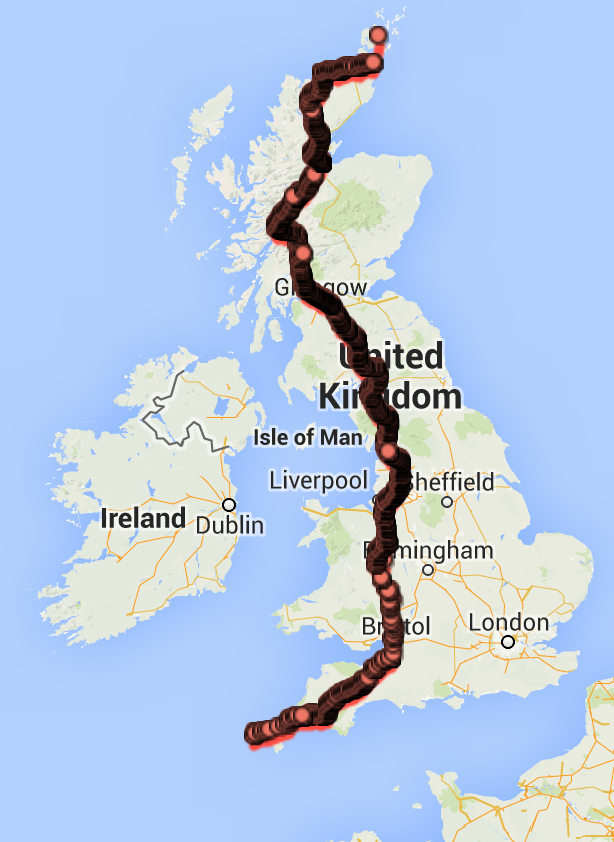
\includegraphics[height=15cm]{lejog-all}
    \end{center}

\end{slide}


\begin{slide}

    \textcolor{blue}{\Large{LEJOG Map}}

    \begin{center}
        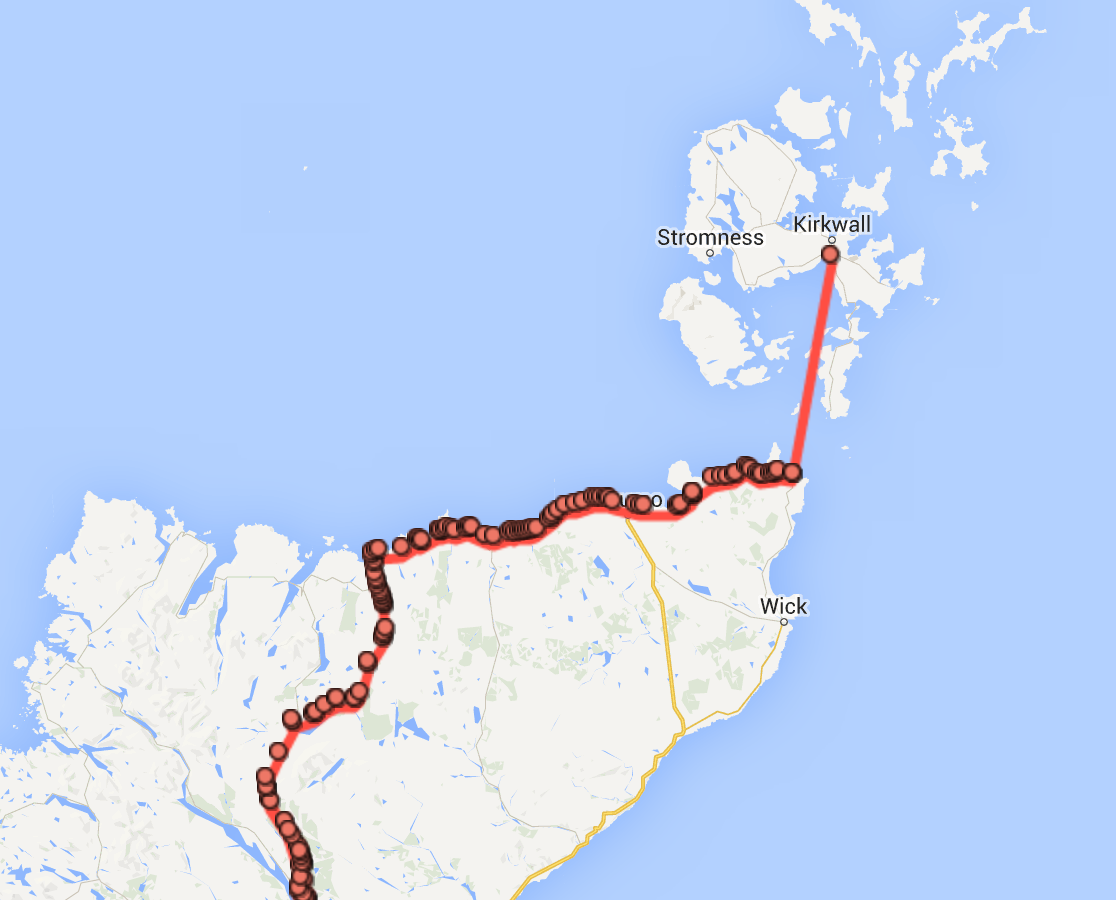
\includegraphics[height=15cm]{lejog-screwed}
    \end{center}

\end{slide}



\begin{slide}

    \textcolor{blue}{\Large{LEJOG Map}}

    \begin{center}
        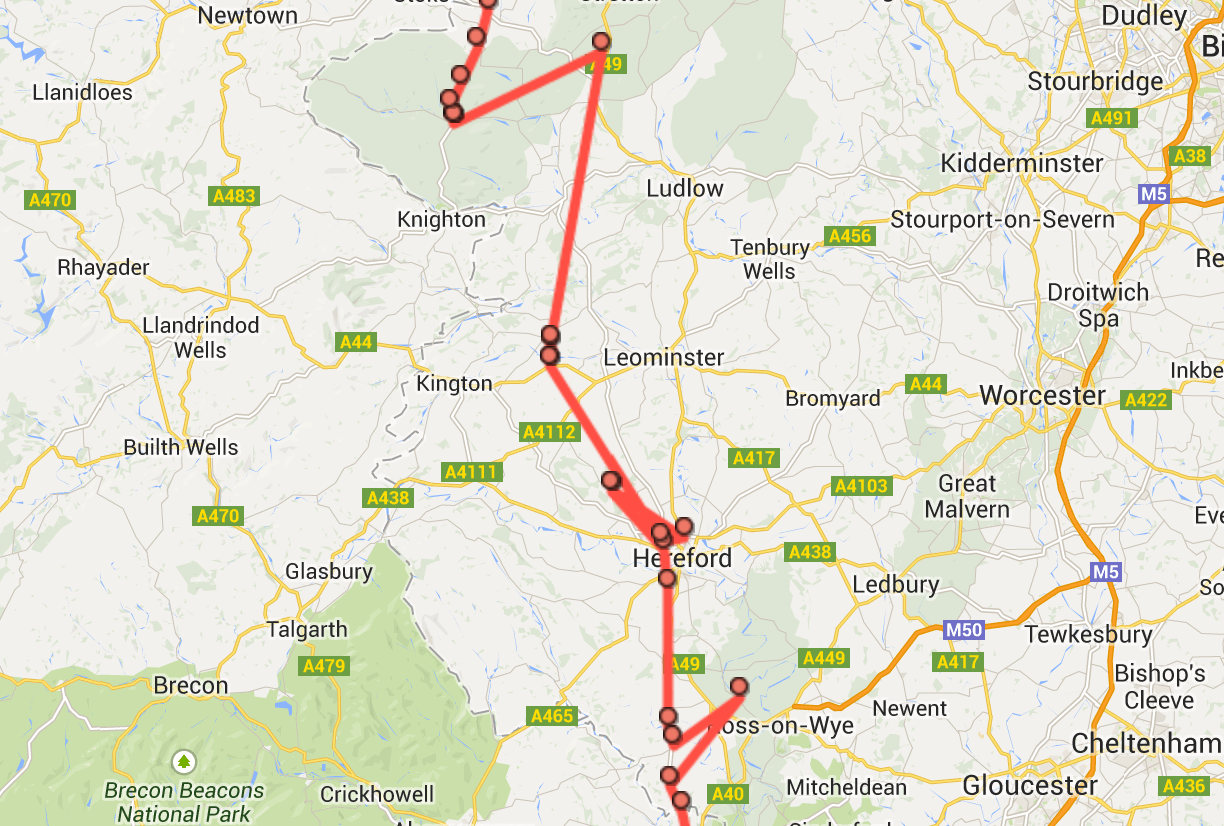
\includegraphics[height=15cm]{lejog-sparse}
    \end{center}

    % can merge with location stamps from photos as Jamie did when he
    % went to Kathmandu

\end{slide}


\begin{slide}

    \textcolor{blue}{\Large{LEJOG Total Stats (Garmin)}}

    \begin{itemize}
        \item 14 days
        \item 1004 miles
        \item 90 hours cycling
        \item 51k feet of elevation gain
        \item 52k calories burnt
        \item Weight before: 77.3kg, after: 77.8kg
    \end{itemize}

\end{slide}


\begin{slide}

    \textcolor{blue}{\Large{LEJOG Lifelogging}}

    \begin{itemize}
        \item Low on time, still want to make sure I record alcohol consumption, inhaler usage
        \item Had to find and use shortcuts...
    \end{itemize}

\end{slide}


% part 2


\begin{slide}

    \textcolor{blue}{\Large{Lifelogger}}

    \begin{itemize}
        \item Google Calendar data storage, re-built as more user-friendly and faster
        \item \url{https://github.com/adamchainz/lifelogger}
    \end{itemize}

\end{slide}


\begin{slide}

    \textcolor{blue}{\Large{Lifelogger Data Flow}}

    \begin{center}
        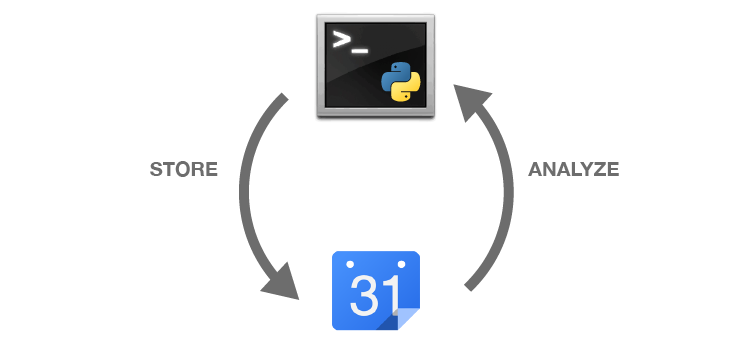
\includegraphics[height=10cm]{lifelog-input-basic}
    \end{center}

\end{slide}


\begin{slide}

    \textcolor{blue}{\Large{Lifelogger Data Flow}}

    \begin{center}
        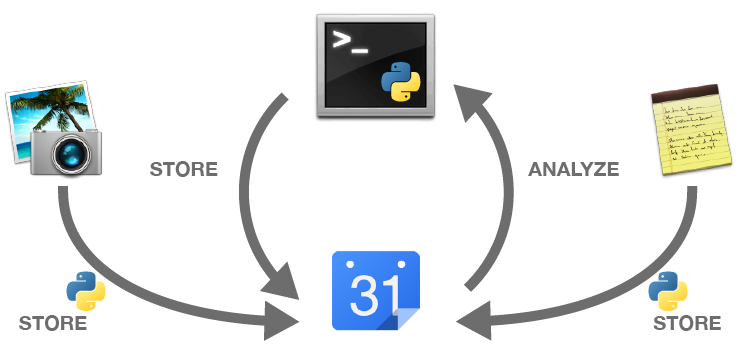
\includegraphics[height=10cm]{lifelog-input-extended}
    \end{center}

\end{slide}


\begin{slide}

    \textcolor{blue}{\Large{Photos}}

    \begin{center}
        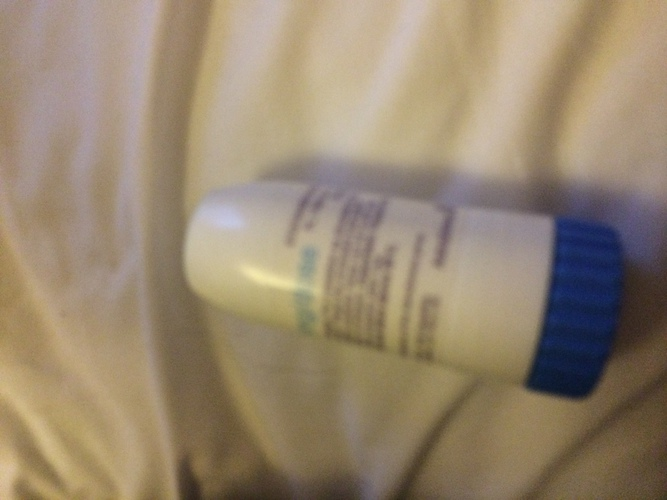
\includegraphics[height=7cm,angle=270]{lifelog-photo-inhaler}
    \end{center}

    \begin{itemize}
        \item \textbf{``Inhaler \#drugs''}
        \item @ 2014-06-11 21:44:03
    \end{itemize}

\end{slide}



\begin{slide}

    \textcolor{blue}{\Large{Photos}}

    \begin{center}
        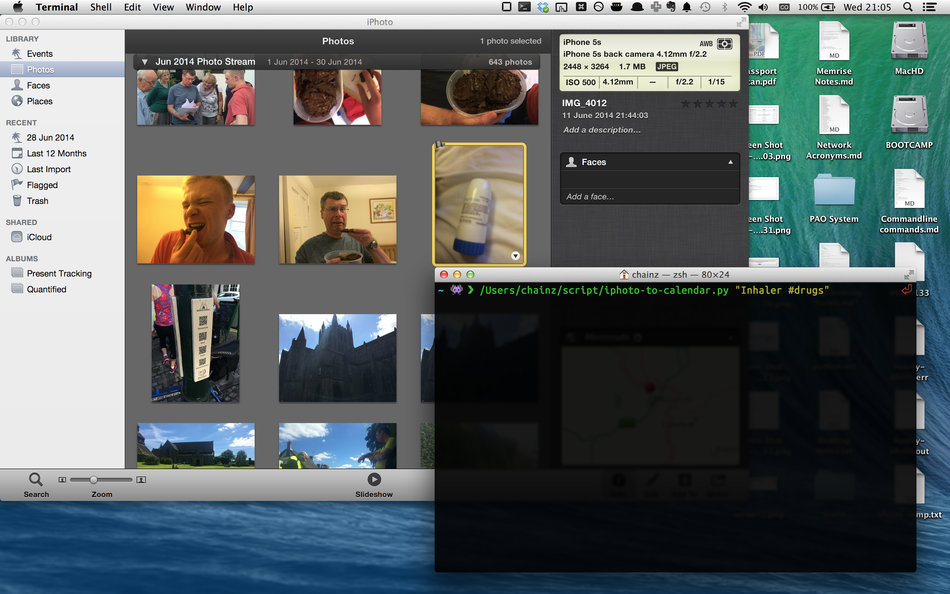
\includegraphics[height=10cm]{lifelog-iphoto-converter}
    \end{center}

    \begin{itemize}
        \item One key press - macro opens terminal, runs \textbf{lifelogger}, my script gets timestamp, adds event to calendar, trashes in iPhoto

    \end{itemize}

\end{slide}


\begin{slide}

    \textcolor{blue}{\Large{Notes}}

    \begin{center}
        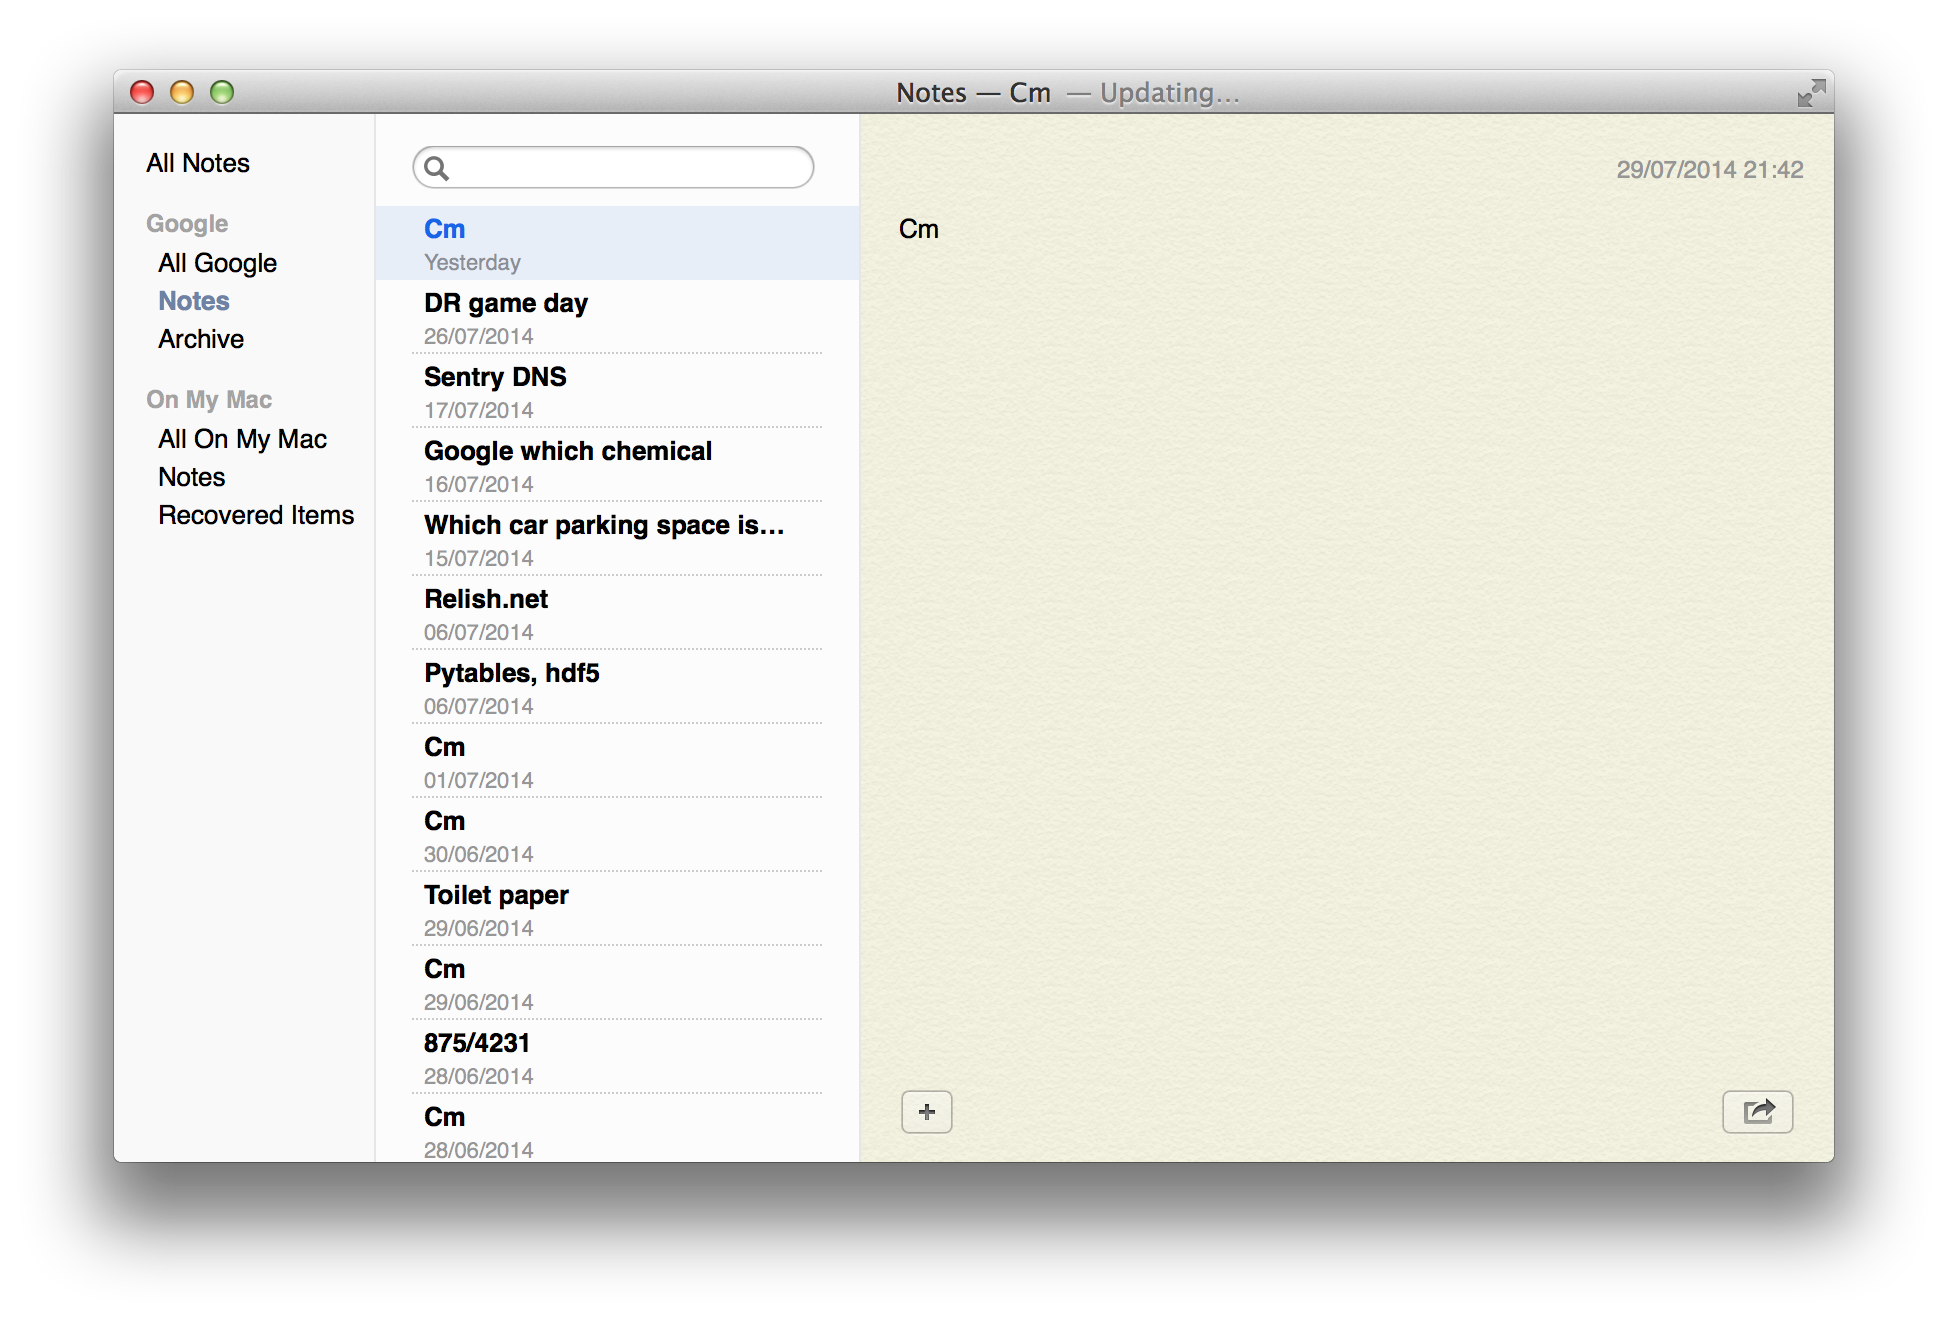
\includegraphics[height=12cm]{lifelog-notes}
    \end{center}

    \begin{itemize}
        \item Same deal - simple notes, less phone space
    \end{itemize}

\end{slide}


% part 2


\begin{slide}

    \textcolor{blue}{\Large{Lifelogger}}

    \begin{center}
        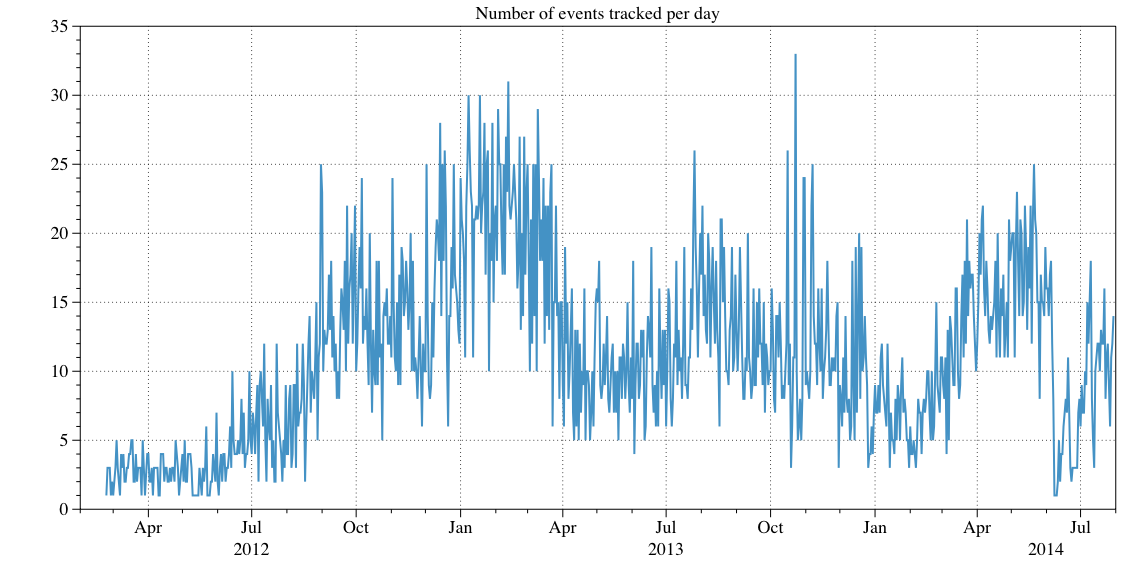
\includegraphics[height=12cm]{lifelog-number-per-day}
    \end{center}

\end{slide}



\begin{slide}

    \textcolor{blue}{\Large{Lifelogger Asthma}}

    \begin{center}
        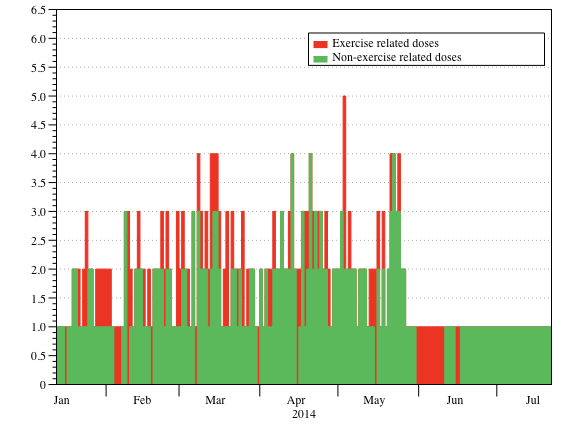
\includegraphics[height=12cm]{lifelog-inhalers}
    \end{center}

\end{slide}




% \begin{slide}

%     \textcolor{blue}{\Large{Powerbreathe}}

%     \begin{itemize}
%         \item (picture)
%         \item Claims to help improve breathing...
%         \item ...but does it?
%     \end{itemize}

% \end{slide}



% \begin{slide}

%     \textcolor{blue}{\Large{Powerbreathe Chart}}

%     \begin{itemize}
%         \item Num times done per day PLUS peakflow record
%     \end{itemize}

%     % so, it probably doesn't

% \end{slide}




% part 3

\begin{slide}

    \textcolor{blue}{\Large{Lift}}

    \begin{center}
        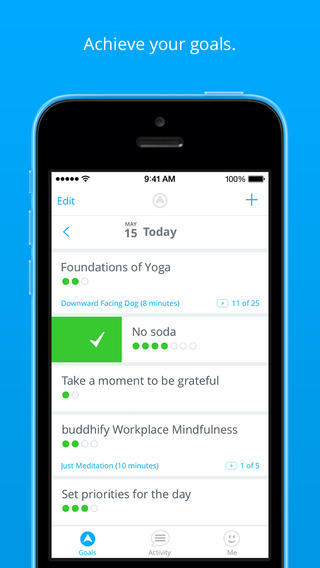
\includegraphics[width=8cm]{lift}
    \end{center}

\end{slide}

\begin{slide}

    \textcolor{blue}{\Large{Lift}}

    \begin{itemize}
        \item Great for quotidian activity tracking
        \item Was going to code similar myself via my lifelog - easier
              to use an existing tool with social side...
        \item ..but I did make sure it had data export before I started using it :)
    \end{itemize}

\end{slide}


\begin{slide}

    \textcolor{blue}{\Large{Lift Analysis}}

    \begin{center}
        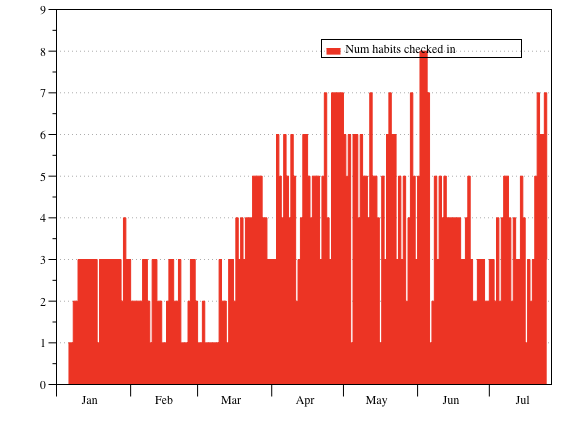
\includegraphics[height=14cm]{lift-checkins}
    \end{center}

\end{slide}


\begin{slide}

    \textcolor{blue}{\Large{Lift Analysis}}

    \begin{center}
        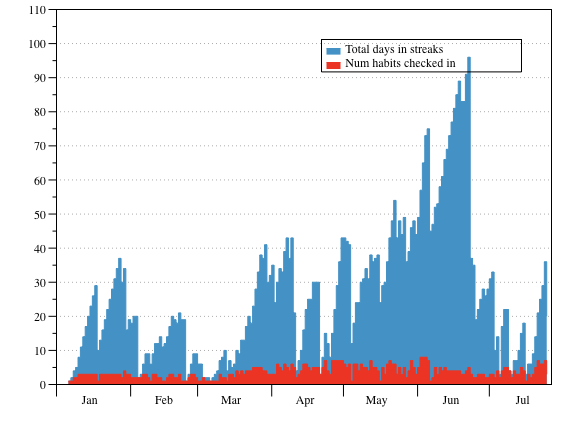
\includegraphics[height=14cm]{lift-checkins-and-streaks}
    \end{center}

\end{slide}


\begin{slide}

    \textcolor{blue}{\Large{Lift Analysis}}

    \begin{center}
        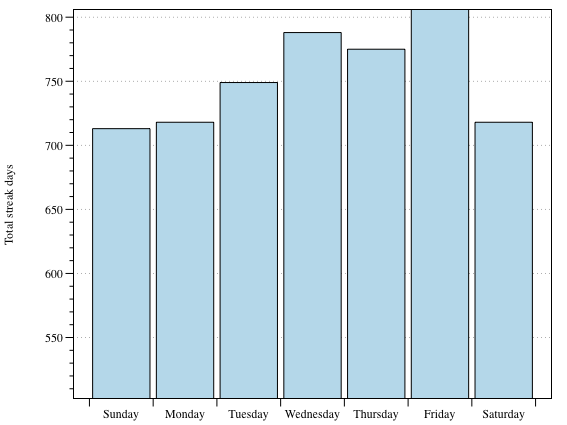
\includegraphics[height=14cm]{lift-group-day}
    \end{center}

\end{slide}


\begin{slide}
    \textcolor{blue}{\Large{Thank you}}

    \begin{itemize}
        \item \url{me@adamj.eu}
    \end{itemize}

\end{slide}

\end{document}
